\documentclass[14pt,a4paper,report]{report}
\usepackage[a4paper, mag=1000, left=2.5cm, right=1cm, top=2cm, bottom=2cm, headsep=0.7cm, footskip=1cm]{geometry}
\usepackage[utf8]{inputenc}
\usepackage[english,russian]{babel}
\usepackage{indentfirst}
\usepackage[dvipsnames]{xcolor}
\usepackage[colorlinks]{hyperref}
\usepackage{listings} 
\usepackage{fancyhdr}
\usepackage{caption}
\usepackage{amsmath}
\usepackage{latexsym}
\usepackage{graphicx}
\usepackage{amsmath}
\usepackage{booktabs}
\usepackage{array}
\hypersetup{
	colorlinks = true,
	linkcolor  = black
}

\usepackage{titlesec}
\titleformat{\chapter}
{\Large\bfseries} % format
{}                % label
{0pt}             % sep
{\huge}           % before-code


\DeclareCaptionFont{white}{\color{white}} 

% Listing description
\usepackage{listings} 
\DeclareCaptionFormat{listing}{\colorbox{gray}{\parbox{\textwidth}{#1#2#3}}}
\captionsetup[lstlisting]{format=listing,labelfont=white,textfont=white}
\lstset{ 
	% Listing settings
	inputencoding = utf8,			
	extendedchars = \true, 
	keepspaces = true, 			  	 % Поддержка кириллицы и пробелов в комментариях
	language = Matlab,            	 	 % Язык программирования (для подсветки)
	basicstyle = \small\sffamily, 	 % Размер и начертание шрифта для подсветки кода
	numbers = left,               	 % Где поставить нумерацию строк (слева\справа)
	numberstyle = \tiny,          	 % Размер шрифта для номеров строк
	stepnumber = 1,               	 % Размер шага между двумя номерами строк
	numbersep = 5pt,              	 % Как далеко отстоят номера строк от подсвечиваемого кода
	backgroundcolor = \color{white}, % Цвет фона подсветки - используем \usepackage{color}
	showspaces = false,           	 % Показывать или нет пробелы специальными отступами
	showstringspaces = false,    	 % Показывать или нет пробелы в строках
	showtabs = false,           	 % Показывать или нет табуляцию в строках
	frame = single,              	 % Рисовать рамку вокруг кода
	tabsize = 2,                  	 % Размер табуляции по умолчанию равен 2 пробелам
	captionpos = t,             	 % Позиция заголовка вверху [t] или внизу [b] 
	breaklines = true,           	 % Автоматически переносить строки (да\нет)
	breakatwhitespace = false,   	 % Переносить строки только если есть пробел
	escapeinside = {\%*}{*)}      	 % Если нужно добавить комментарии в коде
}

\begin{document}

\def\contentsname{Содержание}

% Titlepage
\begin{titlepage}
	\begin{center}
		\textsc{Санкт-Петербургский Политехнический 
			Университет Петра Великого\\[5mm]
			Кафедра компьютерных систем и программных технологий}
		
		\vfill
		
		\textbf{Курсовая работа\\[3mm]
			Курс: «Администрирование компьютерных сетей»\\[3mm]
			Тема: «Проектирование корпоративной компьютерной сети для фирмы по юридической консультации»\\[35mm]
			}
	\end{center}
	
	\hfill
	\begin{minipage}{.5\textwidth}
		Выполнил студент:\\[2mm] 
		Ерниязов Тимур Ертлеуевич\\
		Группа: 13541/2\\[5mm]
		
		Проверил:\\[2mm] 
		Малышев Игорь Алексеевич
	\end{minipage}
	\vfill
	\begin{center}
		Санкт-Петербург\\ \the\year\ г.
	\end{center}
\end{titlepage}

% Contents
\tableofcontents
\clearpage


\section*{Введение}
В современном мире работа ни одной организации не обходится без помощи сети. Люди
всегда стремились сделать свою жизнь проще. Нехватка времени явилась причиной
научно технического прогресса, создания различной техники, благодаря работе
которой человек мог значительно быстрее решать поставленные перед ним задачи.

Работа сети во многом зависит от рациональной структуры её реализации, то есть актуальным до сих пор является вопрос построения сети. Эта задача и является целью создания данной работы.

\section{Цель работы}
Создать и настроить компьютерную сеть для фирмы юридической консультации средствами \textbf{Cisco Packet Tracer}. Установить и сконфигурировать необходимые сервисы. Выполнить проверку работы сети.

\section{Постановка задачи}
\textbf{Разрабатываемая сеть должна отвечать следующим требованиям:}
\begin{enumerate}
\item Иметь несколько подсетей:
\begin{itemize}
\item Пользовательская (для сотрудников);
\item Подсеть с сайтом компании и почтовым сервисом;
\item Служебная подсеть, в которой хранятся рабочие файлы компании.
\end{itemize}
\item Пользовательская сеть должна иметь доступ к другим подсетям, а также к сети "интернет";
\item Служебная подсеть должна быть изолирована от сети "интернет".
%\item Масштабирование, с минимальными правками в сети.
\end{enumerate}
\textbf{Реализуемая функциональность подсетей:}
\begin{enumerate}
\item Пользовательская (для сотрудников):
\begin{itemize}
\item Настроенный DHCP сервер, для автоматического получения адреса сотрудниками.
\end{itemize}
\item Подсеть с сайтом компании:
\begin{itemize}
\item Email и HTTP сервер с сайтом комании.
\end{itemize}
\item Служебная подсеть:
\begin{itemize}
\item TFTP сервер для хранения файлов.
\end{itemize}
\end{enumerate}


\section{Выполнение работы}

\subsection{Создание сети}
Для создания сети, были исспользованы следующие элементы Cisco Packet Tracer:
\begin{itemize}
\item Конечные устройства:
\begin{itemize}
\item \textbf{PC-PT} - компьютер;
\item \textbf{Server-PT} - сервер;
\end{itemize}
\item Сетевые устройства:
\begin{itemize}
\item \textbf{Router-PT} - роутер;
\item \textbf{2950-24} - коммутатор на 24 порта;
\end{itemize}
\end{itemize}
Связь между устройствами была произведена с использованием инструмента \textbf{automatically choose connection type}, который автоматически подключает интерфейсы устройств.

Была спроектирована следующая сеть, приведенная на рисунке 1.

\begin{figure}[h]
  \centering
  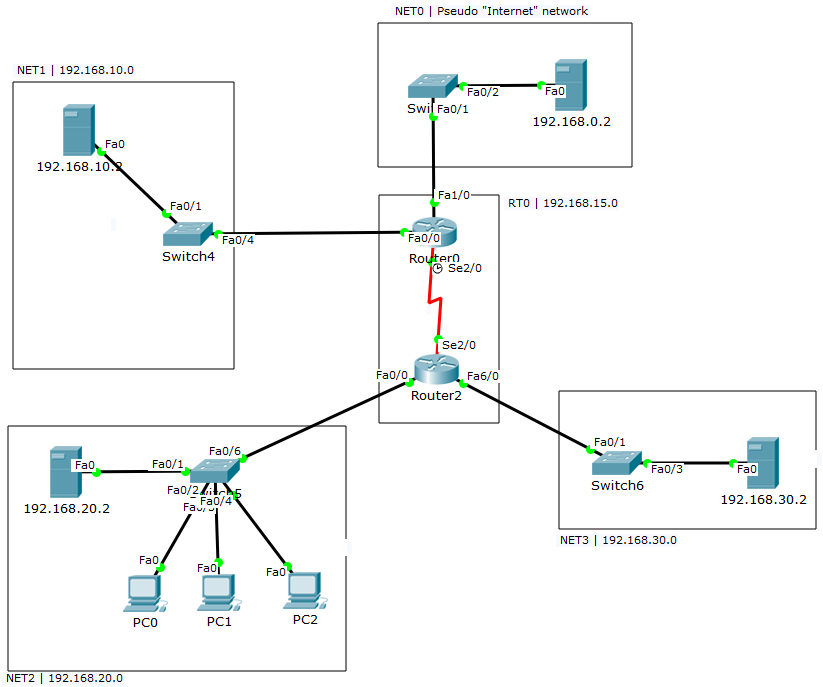
\includegraphics[width=.8\textwidth]{img/scheme}
  \caption{Вкладка Desktop}
\end{figure}
Представленную сеть можно разделить на следующие подсети:
\begin{itemize}
\item \textbf{NET0} - сеть имитирующая работу сети "интернет", необходима, так как Cisco Packet Tracer не предоставляет возможность доступа к реальной сети;
\item \textbf{NET1} - Подсеть с сайтом компании;
\item \textbf{NET2} - Пользовательская (для сотрудников) подсеть;
\item \textbf{NET3} - Служебная подсеть;
\item \textbf{RT0} - Подсеть для свзи роутеров. Связь выполнена с помощью порта \textbf{serial}. Подобный тип подключения является устаревшим, но другого выбора подключения двух роутеров в программе не представлено, поэтому можно считать это особенностью Cisco Packet Tracer.
\end{itemize}
\clearpage

\subsection{Настройка подсети NET0 (имитация внешней сети)}
\subsubsection{Конфигурирование интерфейсов}
В подсети находится один конечный узел. Для настройки интерфейса выберм узел и перейдем на вкладку \textbf{Desktop}
\begin{figure}[h]
  \centering
  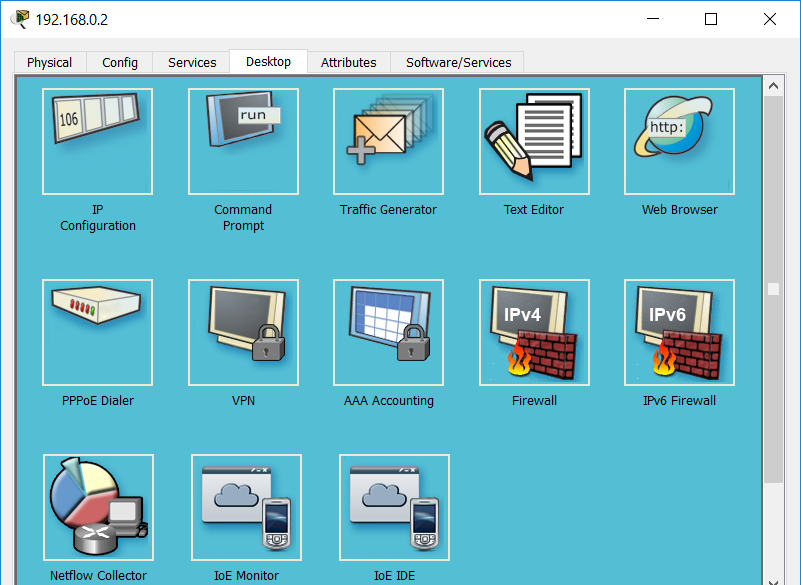
\includegraphics[width=.6\textwidth]{img/net0_0_2__0}
  \caption{Вкладка Desktop}
\end{figure}

Во вкладке представлены различные утилиты. Для настройки интерфейса необходимо выбрать \textbf{IP Configuration}

\begin{figure}[h]
  \centering
  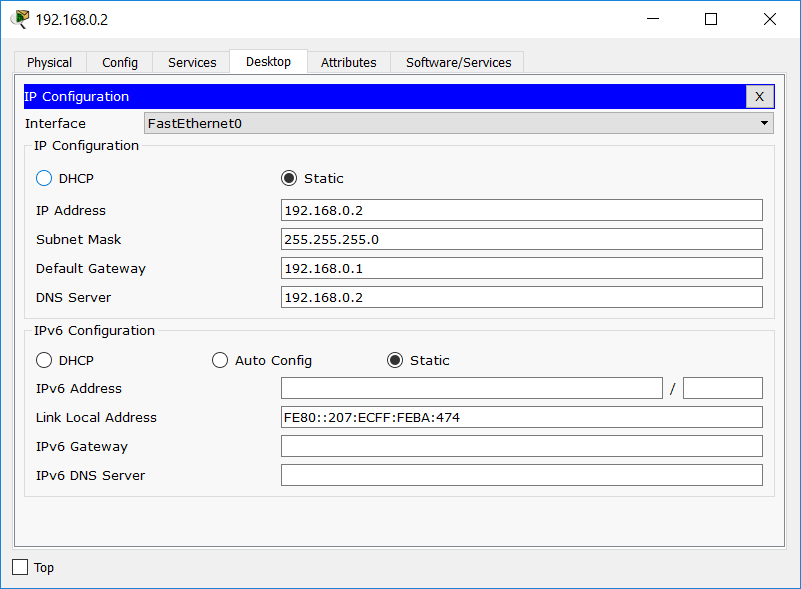
\includegraphics[width=.6\textwidth]{img/net0_0_2__1}
  \caption{Сконфигурированный интерфейс FastEthernet0}
\end{figure}

Интерфейс был сконфигурирован статически. Адрес \textbf{192.168.0.1} является интерфейсом роутера, к которому имеется подключение через коммутатор. В качестве DNS сервера выступает этот же конечный узел.
\subsubsection{Установка и настройка сетевых сервисов}
Доступные сервисы находятся на вкладке \textbf{Services}. Для добавления новой записи необходимо указать \textbf{Name} - доменное имя, и \textbf{Address} - адрес ресурса.

\begin{figure}[h]
  \centering
  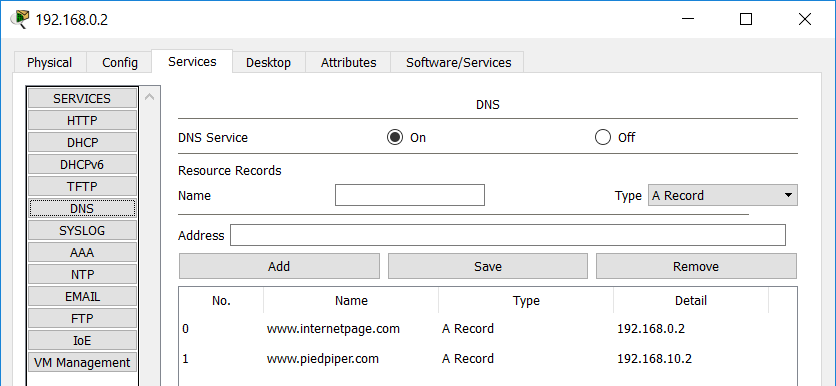
\includegraphics[width=.7\textwidth]{img/net0_0_2__2}
  \caption{Сконфигурированный DNS сервис}
\end{figure}


Было добавлено 2 записи:
\begin{enumerate}
\item \textbf{www.internetpage.com} - имитация сайта в сети "интернет";
\item \textbf{www.urcons.com} - сайт компании.
\end{enumerate}


В конечных узлах типа - сервер, по умолчанию включен HTTP сервис, в котором по умолчанию уже имеются некоторые файлы для работы сайта. Формат web страницы - \textbf{html}, что означает возможность использования html-тегов при редактировании сайта.


\begin{figure}[h]
  \centering
  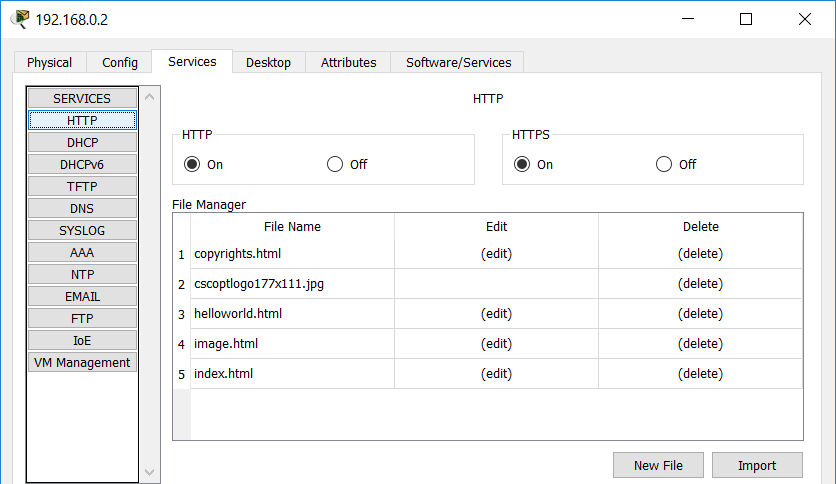
\includegraphics[width=.7\textwidth]{img/net0_0_2__4}
  \caption{HTTP сервис}
\end{figure}
\clearpage

Откроем утилиту - \textbf{Web Browser} и введем в строчке адреса - \textbf{www.internetpage.com}. 

\begin{figure}[h]
  \centering
  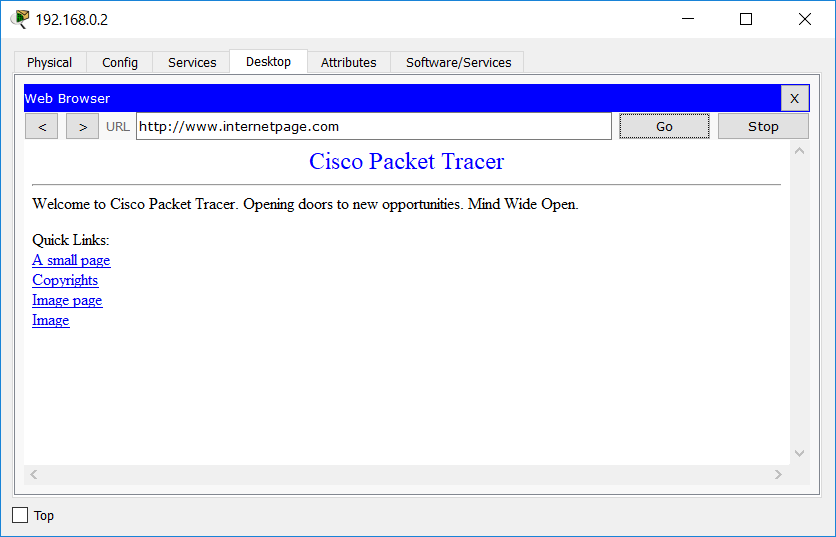
\includegraphics[width=.7\textwidth]{img/net0_0_2__5}
  \caption{WEB страница}
\end{figure}


Для доменного имени был успешно определен адрес, и web страница успешно загрузилась.


\subsection{Настройка подсети NET1 (сеть с сайтом компании)}
\subsubsection{Конфигурирование интерфейсов}
Интерфейс(Fa0) был задан статически:
\begin{itemize}
\item \textbf{IP Address} - 192.168.10.2;
\item \textbf{Subnet Mask} - 255.255.255.0
\item \textbf{Default Gateway} - 192.168.10.1;
\item \textbf{DNS Server} - 192.168.0.2.
\end{itemize}
\subsubsection{Установка и настройка сетевых сервисов}
Был настроен HTTP сервис, но в отличии от настройки в подсети NET0.

Cтраница представляет собой сайт-визитку компании. Доступ к странице также возможен по доменному имени \textbf{www.urcons.com}

\textbf{Примечание:} в случае ввода в редактор кириллических символов, утилита \textbf{Web Browser} отобразит их некорректно.\\\\

\clearpage

Также был настроен Email сервис.
\begin{figure}[h]
  \centering
  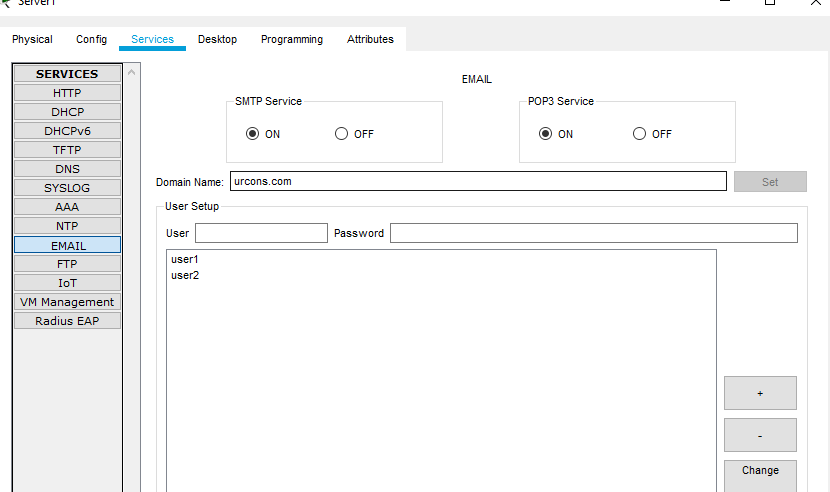
\includegraphics[width=.8\textwidth]{img/4}
  \caption{Email сервис}
\end{figure}
В котором:
\begin{itemize}
\item Указано доменное имя - \textbf{urcons.com};
\item Добавлено 2 пользователя: user1, user2 с паролями password1, password2 соответственно.
\end{itemize}

\subsection{Настройка подсети NET2 (пользовательская сеть)}
\subsubsection{Конфигурирование интерфейсов}
Интерфейс сервера(Fa0) был задан статически:
\begin{itemize}
\item \textbf{IP Address} - 192.168.20.2;
\item \textbf{Subnet Mask} - 255.255.255.0
\item \textbf{Default Gateway} - 192.168.20.1;
\item \textbf{DNS Server} - 192.168.0.2.
\end{itemize}
У всех прочих узлов, в настройках \textbf{IP Configuration} выбирается настройка по DhCP.
\subsubsection{Установка и настройка сетевых сервисов}
Сервис DhCP был включен на сервере (192.168.20.2), где были заполнены следующие поля:
\begin{itemize}
\item \textbf{Interface} - FastEthernet0;
\begin{itemize}
\item единственный интерфейс данного узла.
\end{itemize}
\item \textbf{Default Gateway} - 192.168.20.1;
\begin{itemize}
\item шлюзом по умолчанию выступает интерфейс роутера, подключенный к данной(NET\_2) подсети.
\end{itemize}
\item \textbf{DNS Server} - 192.168.0.2;
\begin{itemize}
\item предварительно настроенный DNS серверс из подсети NET\_0.
\end{itemize}
\item \textbf{Start IP Address} - 192.168.20.5;
\begin{itemize}
\item начала диапазона по выдаче IP-адресов.
\end{itemize}
\item \textbf{Subnet Mask} - 255.255.255.0;
\begin{itemize}
\item маска подсети.
\end{itemize}
\item \textbf{Maximun number of Users} - 100;
\begin{itemize}
\item максимальное количество пользователей.
\end{itemize}
\end{itemize}
На клиентских узлах, с помощью утилиты \textbf{Email} был настроен доступ к Email серверу компании.
\begin{figure}[h]
  \centering
  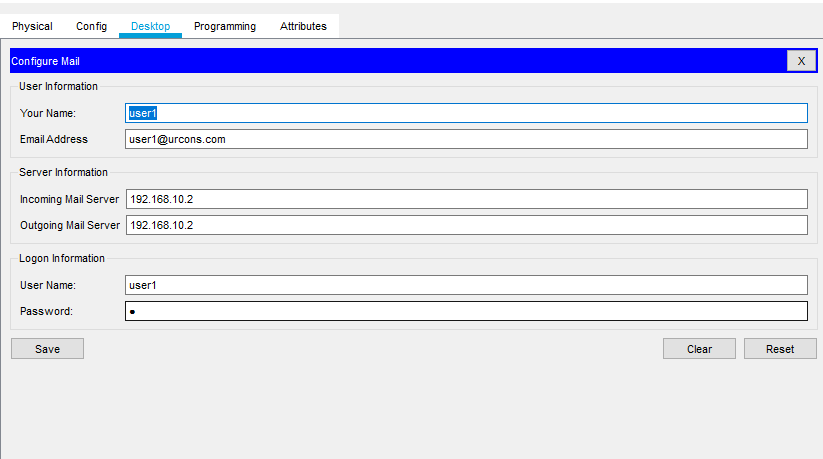
\includegraphics[width=.8\textwidth]{img/3}
  \caption{Настройка доступа к Email серверу на одном из пользовательских узлов}
\end{figure}

\subsection{Настройка подсети NET3 (служебная сеть)}
\subsubsection{Конфигурирование интерфейсов}
Интерфейс сервера(Fa0) был задан статически:
\begin{itemize}
\item \textbf{IP Address} - 192.168.30.2;
\item \textbf{Subnet Mask} - 255.255.255.0
\item \textbf{Default Gateway} - 192.168.30.1;
\item \textbf{DNS Server} - 192.168.0.2.
\end{itemize}
\subsubsection{Установка и настройка сетевых сервисов}
Настройка TFTP сервиса была произведена на вкладке \textbf{Services}. Где его необходимо было включить, и для удобства удалить предварительно сгенерированные в нем файлы.

\subsection{Настройка подсети RT0}
\subsubsection{Конфигурирование интерфейсов}
В сети имеются два роутера(\textbf{Router 0} и \textbf{Router2}), которые выполняют функцию связующего звяна между подсетями.

\subsubsection{Настройка маршрутизации}
Также, для корректной работы сети была добавлена маршрутизация. Для этого на Router 0, в настройках был выбран пункт \textbf{RIP Routing}, в который были добавлены следующие подсети:
\begin{itemize}
\item 192.168.0.0;
\item 192.168.10.0;
\item 192.168.15.0.
\end{itemize}
И для Router 2 соответственно:
\begin{itemize}
\item 192.168.15.0;
\item 192.168.20.0;
\item 192.168.30.0.
\end{itemize}
\subsubsection{Изоляция сети}
Сеть NET3 необходимо изолировать от какого-либо внешнего доступа, то-есть доступ к ней должны иметь сотрудники, из пользовательской сети NET2.

Для этого, на Router2 открывается \textbf{CLI}(Command Line Interface). В котором, для настройки \textbf{ACL}, вводятся следующие команды:
\begin{lstlisting}[language={}, caption={index.html}]
Router> enable
Router# conf terminal

Router(config)#access-list 101 permit ip any 192.168.20.0 0.0.0.255
Router(config)#access-list 101 permit ip 192.168.20.0 0.0.0.255 any
/*Выход из настройки нажатием CTRL + Z*/
Router(config)#^Z
Router#sh access-list
Extended IP access list 101
    10 permit ip any 192.168.20.0 0.0.0.255
    20 permit ip 192.168.20.0 0.0.0.255 192.168.30.0 0.0.0.255
\end{lstlisting}
\begin{itemize}
\item Командой \textbf{enable} был совершен переход в превелигированный режим;
\item Командой \textbf{conf terminal} начата настройка;
\end{itemize}
Командами
\begin{center}
\textbf{access-list 101 permit ip any 192.168.20.0 0.0.0.255}\\
\textbf{access-list 101 permit ip 192.168.20.0 0.0.0.255 any}
\end{center}
и был ограничен доступ всем, кроме пользовательской сети.

Разберем данную команду:
\begin{itemize}
\item \textbf{101} - означает номер правила. 0-99 - обычные правила, 100-199 расширенные. У расширенных правил, разумеется больший диапазон настройки;
\item \textbf{permit} - действие которое будет применено, в данном случае разрешение;
\item \textbf{ip} - тип протокола;
\item \textbf{any 192.168.20.0 0.0.0.255} - любая сеть может обращаться к сети NET2;
\item \textbf{192.168.20.0 0.0.0.255 any} - сеть NET2 может обращаться к любой сети.
\end{itemize}
По умолчанию, все пакеты разрешены(permit), но после включения правил \textbf{ACL}, к пакетам которые не подходят не под одно правило, будет применено действие \textbf{deny}, то есть они не будут пропущены.

Таким образом, для сети NET3, был сохранен доступ из пользовательской сети, и в тоже время ограничен доступ из прочих сетей


\section{Тестирование}
\subsection{Проверка Email сервера}
От пользователя \textbf{user2@urcons.com} создается письмо пользователю \textbf{user1@urcons.com}. Для отправки необходимо нажать кнопку \textbf{Send}.

Зайдем в утилиту \textbf{Email} от пользователя \textbf{user1@urcons.com}, и получим почту кнопкой \textbf{Receive}.
\clearpage
\begin{figure}[h]
  \centering
  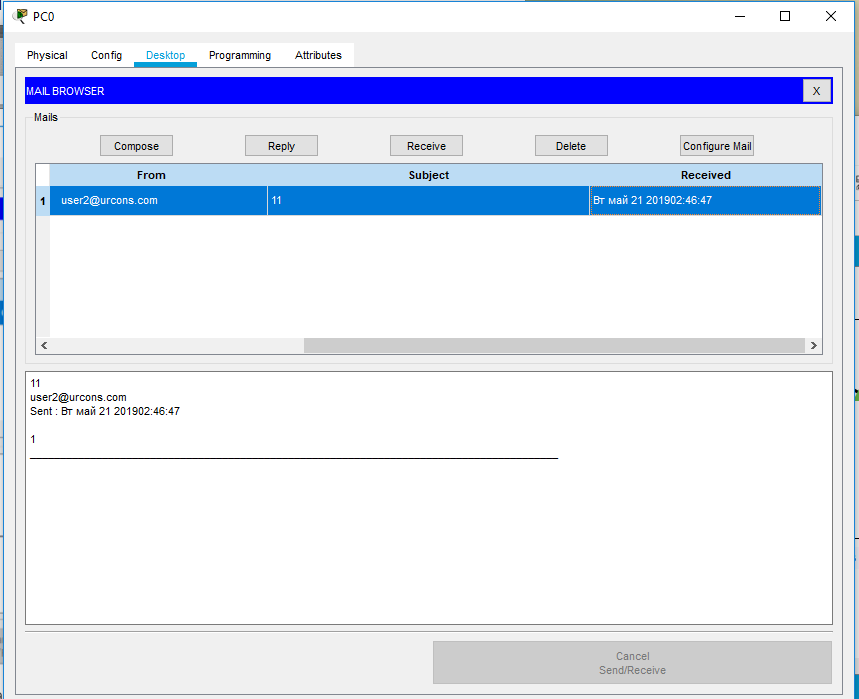
\includegraphics[width=.8\textwidth]{img/1}
  \caption{Получение письма}
\end{figure}
В списке писем появилось, отправленное ранее, письмо. Также имеется дополнительная информация: дата отправки, протокол по которому письмо было получено, адрес сервера почты. 

\subsection{Проверка TFTP}
На Router 2 была открыта консоль, в которой были выполнены следующие команды:
\begin{lstlisting}[language={}]
Router>enable
Router#show flash

System flash directory:
File  Length   Name/status
  3   5571584  pt1000-i-mz.122-28.bin
  2   28282    sigdef-category.xml
  1   227537   sigdef-default.xml
[5827403 bytes used, 58188981 available, 64016384 total]
63488K bytes of processor board System flash (Read/Write)

Router#copy flash tftp
Source filename []? pt1000-i-mz.122-28.bin
Address or name of remote host []? 192.168.30.1
Destination filename [pt1000-i-mz.122-28.bin]? temp.file

Writing pt1000-i-mz.122-28.bin...!!!!!!!!!!!!!!!!!!!!!!
[OK - 5571584 bytes]

5571584 bytes copied in 0.147 secs (8684467 bytes/sec)
\end{lstlisting}
Разберем действия:
\begin{enumerate}
\item Командой \textbf{enable} был совершен переход в привелегированный режим, можно заметить по символу решетки;
\item Командой \textbf{show flash} было выведено содержимое флеш-памяти, в данном случае это необходимо для тестовой загрузки по TFTP;
\item Командой \textbf{copy flash tftp} сообщаем о начале загрузке файла по tftp, где далее указывается файл(ы), tftp сервер для загрузки, а также новое имя файла(ов). 
\end{enumerate}
На TFTP сервере, в настройках TFTP появится выбранный ранее файл с указанным именем.

\subsection{Проверка команды ping по адресу}
Откроем на узле 192.168.20.4(сеть NET2) утилиту \textbf{Command Prompt}, в которой введем команды \textbf{ipconfig} и \textbf{ping} в которой укажем адрес 192.168.0.2(сеть NET0).
\begin{lstlisting}[language={}]
C:\>ipconfig
FastEthernet0 Connection:(default port)
   Link-local IPv6 Address.........: FE80::2E0:A3FF:FEA3:7605
   IP Address......................: 192.168.20.5
   Subnet Mask.....................: 255.255.255.0
   Default Gateway.................: 192.168.20.1

C:\>ping 192.168.0.2
Pinging 192.168.0.2 with 32 bytes of data:
Reply from 192.168.0.2: bytes=32 time=1ms TTL=127
Reply from 192.168.0.2: bytes=32 time=1ms TTL=127
Reply from 192.168.0.2: bytes=32 time=1ms TTL=127
Reply from 192.168.0.2: bytes=32 time<1ms TTL=127

Ping statistics for 192.168.0.2:
    Packets: Sent = 4, Received = 4, Lost = 0 (0% loss),
Approximate round trip times in milli-seconds:
    Minimum = 0ms, Maximum = 1ms, Average = 0ms
\end{lstlisting}
Как видно из лога, команда пинг была успешна.

\subsection{Проверка команды ping по доменному имени}
Откроем на узле 192.168.20.2(сеть NET2) утилиту \textbf{Command Prompt}, в которой введем команды \textbf{ipconfig} и \textbf{ping} в которой укажем доменное имя \textbf{www.mypage.com}.
\begin{lstlisting}[language={}]
C:\>ipconfig
FastEthernet0 Connection:(default port)
   Link-local IPv6 Address.........: FE80::201:42FF:FE0B:D82B
   IP Address......................: 192.168.20.5
   Subnet Mask.....................: 255.255.255.0
   Default Gateway.................: 192.168.20.1

C:\>ping www.urcons.com
Pinging 192.168.10.2 with 32 bytes of data:
Reply from 192.168.10.2: bytes=32 time<1ms TTL=126
Reply from 192.168.10.2: bytes=32 time=10ms TTL=126
Reply from 192.168.10.2: bytes=32 time=11ms TTL=126
Reply from 192.168.10.2: bytes=32 time=13ms TTL=126

Ping statistics for 192.168.10.2:
    Packets: Sent = 4, Received = 4, Lost = 0 (0% loss),
Approximate round trip times in milli-seconds:
    Minimum = 0ms, Maximum = 13ms, Average = 8ms
\end{lstlisting}
Как видно из лога, доменное имя было преобразовано в адрес, по которому и была произведена команда ping.

\subsection{Проверка команды ping из изолированной сети}
Откроем на узле 192.168.30.2(сеть NET3) утилиту \textbf{Command Prompt}, в которой введем команды \textbf{ipconfig} и \textbf{ping} в которой укажем доменное адрес 192.168.0.2(NET0).
\begin{lstlisting}[language={}]
C:\>ipconfig

FastEthernet0 Connection:(default port)

   Link-local IPv6 Address.........: FE80::200:CFF:FECC:E597
   IP Address......................: 192.168.30.2
   Subnet Mask.....................: 255.255.255.0
   Default Gateway.................: 192.168.30.1

C:\>ping 192.168.0.2

Pinging 192.168.0.2 with 32 bytes of data:

Reply from 192.168.30.1: Destination host unreachable.
Reply from 192.168.30.1: Destination host unreachable.
Reply from 192.168.30.1: Destination host unreachable.
Reply from 192.168.30.1: Destination host unreachable.

Ping statistics for 192.168.0.2:
    Packets: Sent = 4, Received = 0, Lost = 4 (100% loss),
\end{lstlisting}
Как видно из лога, благодаря изоляции внешние сети недоступны.
\clearpage
\section{Заключение}
В данной работе был получен опыт по работе в \textbf{Cisco Packet Tracer}(CPT).


Построение и настройка были выполнены с помощью встроенных инструментов, которые в общем виде имитируют реальное оборудование. Если сравнивать построение сети например с WMware, то в нем настройка сети производится на конкретных системах, в то время как в CPT это было сделано на лишь приближенных к реальности устройствах. Однако, решения созданные CPT более легковесны как в настройке, так и в проектировании.

CPT будет полезен как новичкам, так и профессионалам.

Отличительной особенностью является то, что за любым пакетом можно наблюдать по-шагам, что может помочь в определении ситуация, почему сеть работает некорректно.

К недостаткам CPT можно отнести лишь то, что все действия ограничены, то есть установить на устройство какое-либо ПО или сервис которого нет в CPT, не предоставляется возможным.


\end{document}
